
\section{Experiments\label{sec:experiments}}

The experiments evaluate the advantages of a DVS-based tracking solution
with respect to a tracking solution based on a traditional CMOS camera.
We compare the DVS-based \ALM tracking with vision-based tracking
using the PTAM algorithm, using the output of an OptiTrack system
as the ground truth. The data show that the DVS-based tracking is
able to deal with faster motions due to the minimal latency, but the
precision of the reconstructed pose is limited by the low resolution
of the sensor.



\begin{figure}[b]
\centering{}\hfill{}\subfloat[\label{fig:quadcopter_belly}\ALMs configuration]{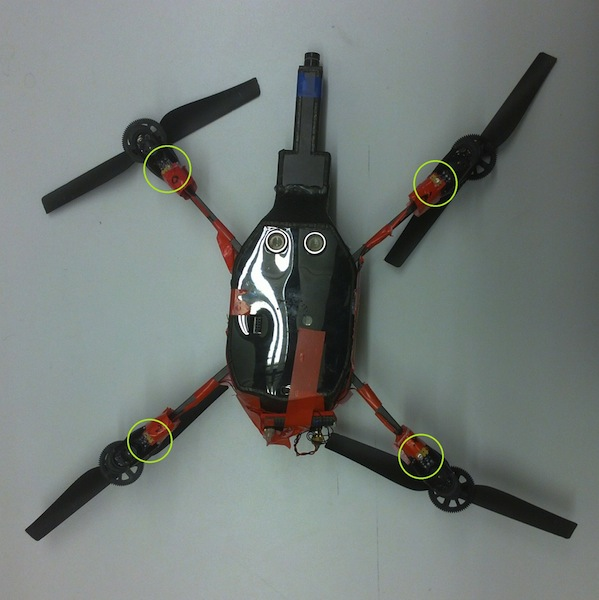
\includegraphics[height=3.5cm]{figures/quadcopter_belly_small} }\hfill{}\subfloat[\label{fig:Infrared-markers-used}Infrared markers]{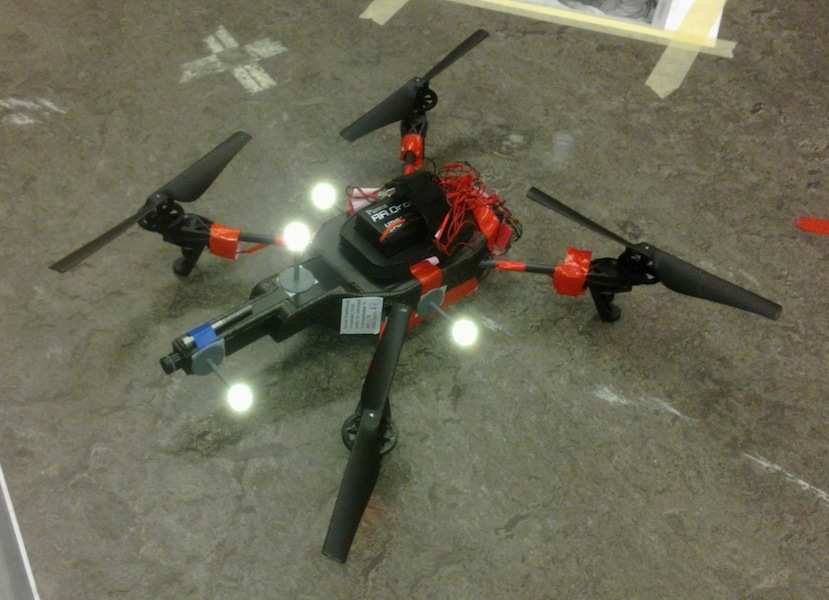
\includegraphics[height=3.5cm]{figures/marked_quadrotor_small}

}\hfill{} \caption{\label{fig:marked_quadrotor}The ARDrone 2.0 equipped with four \ALMs
(shown in \emph{a}) tracked by the DVS, and reflective markers used
by the OptiTrack (shown in \emph{b}). }
\end{figure}



\subsection{Hardware}


\subsubsection{Robot platform}

We used the commercially available ARDrone 2.0. We attached four
custom-built \ALMs to the bottom of the platform (\prettyref{fig:quadcopter_belly}).
Each LED was fixed facing downwards, one under each of the four rotors,
so that the four were lying on a plane forming a square of 20cm side
length. The USB connector available on the drone provided power to
the microcontroller and \ALMs. The drone has also a front-facing
$720\times980$ CMOS camera that is used in these experiments, while
the ground-facing camera is not used.


\subsubsection{DVS}

The DVS128 camera was used for the tests. It has a resolution of $128\times128$
pixels. The lens attached gave the sensor a FOV of approximately 65\textdegree{},
giving a resolution of 0.5~pixels/\textdegree{}. For tracking the
quadcopter, the DVS was installed on the floor facing upwards. Note
that the relative motion between DVS and quadcopter would be the same
if the \ALMs were on the floor and the DVS on board.


\subsubsection{OptiTrack}

To measure the pose estimation accuracy we used a OptiTrack tracking
system from NaturalPoint~\cite{optitrack}, which is a marker-based
optical motion tracking system using active infrared light and reflective
marker balls. Four markers have been applied to the drone (\prettyref{fig:Infrared-markers-used}).
Our lab setup comprised 10 cameras in a $6\times8\,\mbox{m}$ area;
the cost of this system is approximately 20,000~CHF (\$21,000). The
sampling frequency used was $250$~Hz. The manufacturer states that
the accuracy is~$\sim1$~mm, but this seems a rather optimistic
estimate based on our experience with the system; we evaluate the
accuracy to be closer to 5--10~mm.



\begin{figure*}
\begin{centering}

\par\end{centering}

\begin{centering}
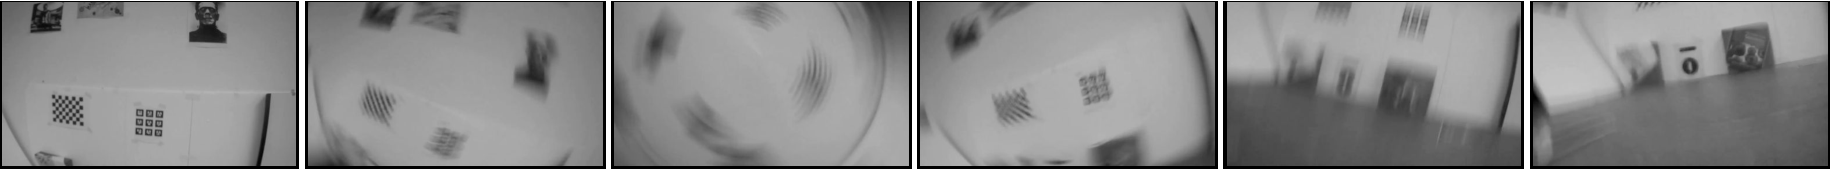
\includegraphics[width=17cm]{figures/slides/flip_sequence_small}
\par\end{centering}

\caption{\label{fig:Motion-blur-induced}Motion blur induced on CMOS image
from flip motion.}
\end{figure*}



\subsubsection{Motion}

The prototypical aggressive maneuver that we use is a ``flip'' of
the quadcopter, i.e. a $360^{\circ}$ roll. During the flip the frontal
camera images are severely blurred (\prettyref{fig:Motion-blur-induced}). 




\subsubsection{Interference OptiTrack / DVS}

We encountered an unexpected incompatibility between OptiTrack and
DVS. The OptiTrack uses high-power infrared spotlights. In the OptiTrack's
standard configuration, the spotlights are pulsed at a high frequency.
This is of course invisible to normal sensors and to the human eye,
but it was a spectacular interference for the DVS. Like most cameras,
the DVS is most sensitive in the infrared spectrum and is much faster
than the OptiTrack strobing frequency. This generated an overflow
in the DVS events buffer as the electronics could not handle the large
number of events to be processed contemporaneously. Eventually we
understood how to deactivate the strobing for all the cameras prior
to recording. Still there was a slight residual interference by the
infrared illumination from the OptiTrack, but it should have relatively
little impact to the results of our experiments.


\subsection{Methods}

We compare three ways to track the pose of the quadcopter: 1)~The
output of our DVS-based \ALM tracking method; 2)~The OptiTrack output;
3)~The output of a traditional feature-based tracker using the data
from the conventional CMOS camera mounted front-facing on the drone.
The image data was streamed to a computer via network interface, were
the parallel tracking and mapping algorithm (PTAM)~\cite{PTAM} was
employed for pose estimation.


\subsubsection{Data recording, synchronization, and alignment\label{sec:datarecording}}

Using this setup we did several recordings, in which we recorded the
OptiTrack tracking data, using its native format, the image data using
a ROS interface, as well as the raw event data from the DVS in the
native format. 

To synchronize the data from different sources we used a motion induced
cue. We moved manually the drone up and down, generating an approximated
sinusoid curve in the position data, which allowed easy manual matching
of the sequences and estimation of the delay between the two.

After adjusting for the delay, we adjusted the sampling frequency.
As our algorithm's output has a lower sampling rate than the OptiTrack
(1~KHz vs 250~Hz), the OptiTrack data was resampled by linear interpolation.



As a final step, the time series were put in the same frame of reference.
Given two sequences of points~$\boldsymbol{x}_{k},\boldsymbol{y}_{k}\in\mathbb{R}^{3}$,
the rototranslation $\left\langle \boldsymbol{R},\boldsymbol{t}\right\rangle \in\mathsf{SE}(3)$
that matches them can be found by solving the optimization problem

\begin{equation}
\begin{aligned}\min_{\left\langle \boldsymbol{R},\boldsymbol{t}\right\rangle \in\mathsf{SE}(3)}\sum_{k}\|\boldsymbol{x}_{k}-(\boldsymbol{R}\boldsymbol{y}_{k}+\boldsymbol{t})\|^{2},\end{aligned}
\label{eq:leastsquares}
\end{equation}
which is a classic Procrustes problem~\cite{gower04procrustes}.




\subsection{Results \label{sec:evaluation}}

We recorded data from 18 flips, of which only 6 were successful. During
the recordings we met a number of unforeseen difficulties due to our
modifications to the drone. Having attached the LEDs and microcontroller
to the drone we found that it had become unstable during flight and
hard to control due to the additional weight, so while it could hover
normally, it did not have enough thrust to stabilize itself after
a flip.




\subsubsection{Tracking downtimes\label{sec:trackingspeed}}

During a flip, both the DVS and PTAM lose tracking: PTAM loses tracking
while the image is blurred; the DVS loses track when the \ALMs are
not visible from the ground. The comparison of these ``blackout times''
gives a direct measurement of the latency of the two systems. 



The length of a flip was measured by considering the roll data from
the OptiTrack, taking the interval between the last measurement before
the flip and the first measurement after the flip when the helicopter
was in a level orientation to the floor. 

To measure the onset and offset of the blackout for the DVS, we considered
the last sample before losing track (i.e. where the interval position
samples were considerably higher than the mean sampling rate) and
the first sample of reacquiring track (regaining a steady sample rate).
The equivalent operation was performed on the PTAM data. 



Table \ref{tab:downtime_tab} shows the mean standard deviation of
the different approaches. Our algorithm lost track during the average
time of 0.35 seconds. PTAM lost track for a mean of 0.8 seconds, which
is more than twice the time of the DVS and takes longer than the average
duration of a flip. One can clearly see that the time where tracking
is lost is much shorter with our approach in respect to PTAM. The
results emphasize that the DVS is faster in recovering lost tracks
than the PTAM approach due to not suffering from motion blur. As verified
with our recordings, the downtimes of the DVS correspond to losing
sight of the LED markers because of their emission angle. With a suitable
configuration of either more markers or dynamic vision sensors, tracking
could be maintained during the whole flip. 

\begin{table}
\caption{\label{tab:downtime_tab} Tracking downtime intervals and the flip
duration.}
\vspace{-2mm}\centering%
\begin{tabular}{r|l}
\rule{0pt}{1em}DVS  & $0.35\pm0.10$ s\tabularnewline
PTAM  & $0.80\pm0.33$ s\tabularnewline
flip duration & $0.56\pm0.15$ s\tabularnewline
\end{tabular}\vspace{-2mm}
\end{table}







\subsubsection{Accuracy of estimated pose\label{sec:poseestimationeval}}

The statistics of the estimation error for DVS and PTAM, considering
the OptiTrack as the ground truth, are summarized in \prettyref{tab:Estimation-error}
and shown in graphical form in~\prettyref{fig:errors}.

As for the translation, the DVS estimation error is roughly two times
lower than PTAM (\prettyref{fig:errors}\emph{a}). Although the spread
of outliers is higher in our approach compared to PTAM, the translation
errors of the latter technique show a broader distribution around
their median. Overall this proves that the DVS approach has higher
accuracy with less spread, if we neglect the extreme tails of the
distribution.

\prettyref{fig:errors}\emph{b}--\emph{d} show the error distribution
for roll, pitch and yaw respectively. The DVS performs worse in roll
and pitch compared to yaw. This was to be expected, because of the
position of the \ALMs. As roll and pitch play a minor roll in quadrotor
pose estimation these can be neglected for finding the drone's orientation.
The DVS performs slightly worse than PTAM with a mean error of 6\textdegree{}
and a deviation of 15\textdegree{} (\prettyref{tab:Estimation-error}).
This is explained by the much lower resolution of the DVS ($128\times128$
pixels) compared to the CMOS camera used by PTAM ($720\times980$
pixels). 

\begin{table}[H]
\caption{\label{tab:Estimation-error}Estimation error of DVS and PTAM compared
to Optitrack}


\centering

\newcommand{\tmean}{mean\xspace}
\newcommand{\incm}{[cm]}
\newcommand{\indeg}{[$^\circ$]}
\newcommand{\tstd}{std.dev.\xspace}
\renewcommand{\tabcolsep}{3pt}
\footnotesize

\begin{tabular}{r|rl|rl|rl|rl}
\multicolumn{1}{r}{} & \multicolumn{2}{c}{(a) Translation} & \multicolumn{2}{c}{(b) Roll } & \multicolumn{2}{c}{(c) Pitch} & \multicolumn{2}{c}{(d) Yaw}\tabularnewline
\cline{2-9} 
DVS\rule{0pt}{1em} & 8.9  & $\pm$ 12.6 cm  & 19  & $\pm$ 27\textdegree{} & 17  & $\pm$ 18\textdegree{}  & 6  & $\pm$ 15\textdegree{}\tabularnewline
PTAM & 19.0 & $\pm$ 12.4 cm & 7  & $\pm$ 22\textdegree{} & 5  & $\pm$ 11\textdegree{}  & 3  & $\pm$ 10\textdegree{}\tabularnewline
\end{tabular}

\end{table}


\begin{figure*}
\begin{centering}
\vspace{-2mm}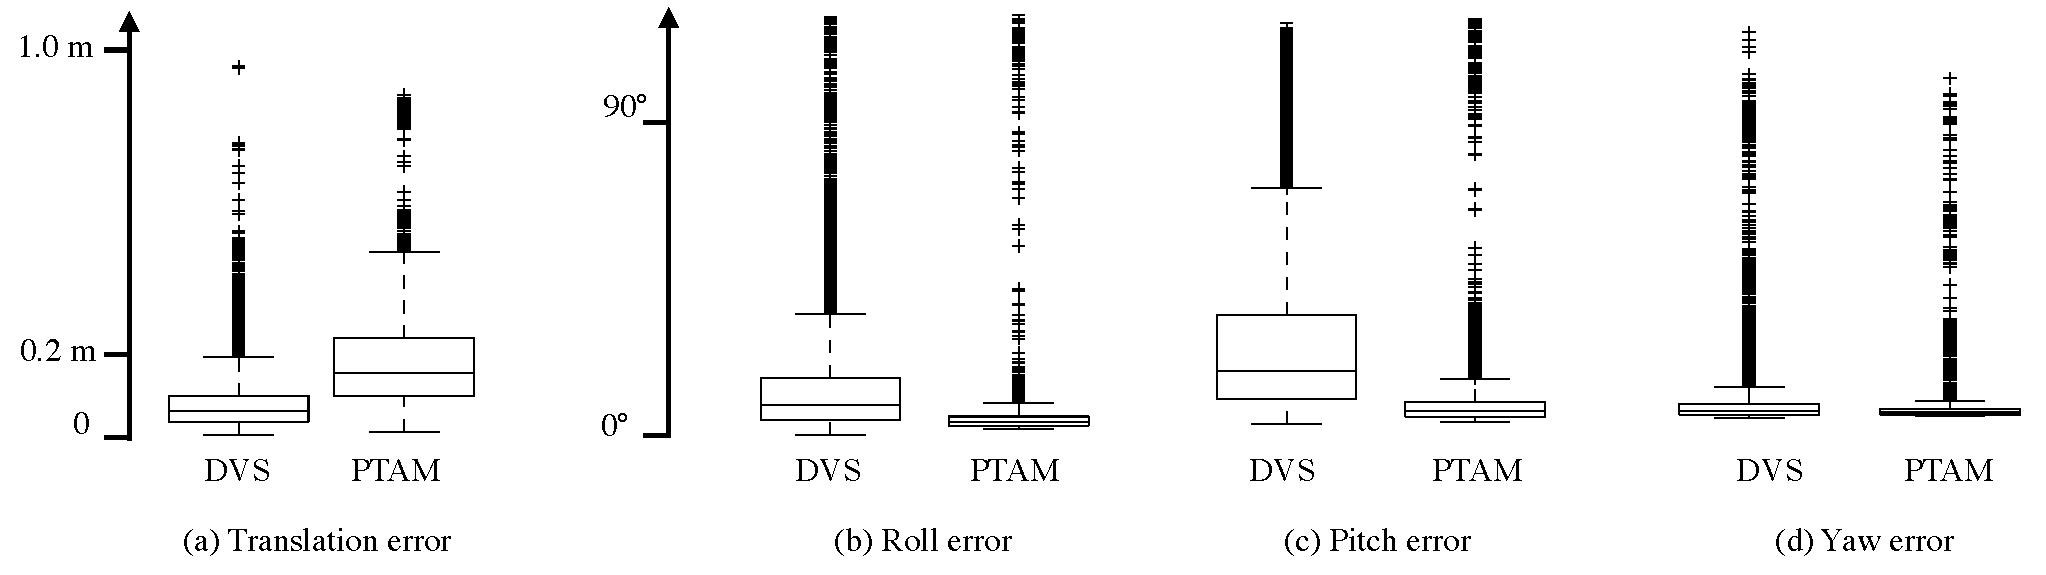
\includegraphics[width=17.5cm]{figures/slides/errors}\vspace{-4mm}
\par\end{centering}

\caption{\label{fig:errors}Distributions of the errors of DVS/PTAM in reference
to the OptiTrack measurements. The data is synthesized in~\prettyref{tab:Estimation-error}.}
\end{figure*}



